\documentclass[../main.tex]{subfiles}






\begin{document}
\chapter{}
\label{cha:cha_13}

\section{}
The data can be tabulated and the sums computed as
	\bigbreak
	\begin{tabular}{cccccccc}
		\Xhline{1.5pt}i&x&y&$x^2$&$x^3$&$x^4$&xy&$x^2y$\\
			\hline1&10&25&100&1000&10000&250&2500\\
			2&20&70&400&8000&160000&1400&28000\\
			3&30&380&900&27000&810000&11400&342000\\
			4&40&550&1600&64000&2560000&22000&880000\\
			5&50&610&2500&125000&6250000&30500&1525000\\
			6&60&1220&3600&216000&12960000&73200&4392000\\
			7&70&830&4900&343000&24010000&58100&4067000\\
			8&80&1450&6400&512000&40960000&116000&9280000\\
			$\Sigma$&360&5135&20400&1296000&87720000&312850&20516500\\
			\Xhline{1.5pt}
	\end{tabular}
	\bigbreak
Normal equations:
	\bigbreak
	$\begin{bmatrix}
		8& 360& 20400\\
		360& 20400& 1296000\\
		20400& 1296000& 87720000\\
	\end{bmatrix}
	\begin{Bmatrix}
		a_0\\
		a_1\\
		a_2\\
	\end{Bmatrix}
	=
	\begin{Bmatrix}
	5135\\
	312850\\
	20516500\\
	\end{Bmatrix}$
	\bigbreak
which can be solved for the coefficients yielding the following best-fit polynomial 
	\bigbreak
$F=-178.4821+16.12202v+0.037202v^2$
	\bigbreak
Here is the resulting fit:
	\bigbreak
	\begin{figure}[H]
		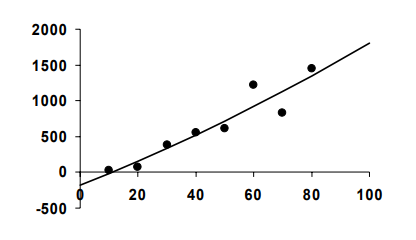
\includegraphics[width=0.5\linewidth]{fig_13_1}
		\label{fig:fig_13_1}
	\end{figure}
	\bigbreak
\begin{blockquote}
The predicted values can be used to determined the sum of the squares. Note that the mean
of the y values is 641.875. 
\end{blockquote}
	\bigbreak
	\begin{tabular}{cccccc}
	\Xhline{1.5pt}i&x&y&$y_{pred}$&$(y_i-\overline{y})^2$&$(y-\overline{y}_{pred})^2$\\
	\hline 10&25&-13.5417&380535&1485\\
	2&20&70&158.8393&327041&7892\\
	3&30&380&338.6607&68579&1709\\
	4&40&550&525.9226&8441&580\\
	5&50&610&720.625&1016&12238\\
	6&60&1220&922.7679&334229&88347\\
	7&70&830&1132.351&35391&91416\\
	8&80&1450&1349.375&\underline{653066}&\underline{10125}\\
	$\Sigma$&&&&1808297&213793\\
	\Xhline{1.5pt}
	\end{tabular}
	\bigbreak
The coefficient of determination can be computed as 
	\bigbreak
$r^2=\dfrac{1808297-213793}{1808297}=0.88177$
	\bigbreak
\begin{blockquote}
The model fits the trend of the data nicely, but it has the deficiency that it yields physically
unrealistic negative forces at low velocities. 
\end{blockquote}
	\bigbreak



\section{}
The sum of the squares of the residuals for this case can be written as
	\bigbreak
$\displaystyle S_r=\sum_{i=1}^{n} (y_{i}-a_{1}x_{i}-a_{2}x_{i}^{2})^{2}$
	\bigbreak
The partial derivatives of this function with respect to the unknown parameters can be
determined as
	\bigbreak
$\displaystyle\dfrac{\delta S_r}{\delta a_1}=-2\sum\big[ (y_{i}-a_{1}x_{i}-a_{2}x_{i}^{2})x_{i}\big]$
	\bigbreak
$\displaystyle\dfrac{\delta S_r}{\delta a_2}=-2\sum\big[ (y_{i}-a_{1}x_{i}-a_{2}x_{i}^{2})x_{i}^{2}\big]$
	\bigbreak
Setting the derivative equal to zero and evaluating the summations gives
	\bigbreak
$\displaystyle\Big(\sum x_{i}^{2}\Big)a_1+\Big(\sum x^{3}_{i}\Big)a_2=\sum x_i y_i$
	\bigbreak
$\displaystyle\Big(\sum x_{i}^{3}\Big)a_1+\Big(\sum x^{4}_{i}\Big)a_2=\sum x_{i}^{2} y_i$
	\bigbreak
which can be solved for
	\bigbreak
$\displaystyle a_1=\dfrac{\sum x_i y_i \sum x_i^4-\sum x^{2}_{i} y_i \sum x^{3}_{i}}{\sum x^{2}_{i} \sum x^{4}_{i} - \Big(\sum x^{3}_{i}\big)^2}$
	\bigbreak
The model can be tested for the data from Table \ref{sec:sec_12_1}.
	\bigbreak
	\begin{tabular}{ccccccc}
	\Xhline{1.5pt}x&y&$x^2$&$x^3$&$x^4$&xy&$x^2y$\\
	\hline10&25&100&1000&10000&250&2500\\
		20&70&400&8000&160000&1400&28000\\
		30&380&900&27000&810000&11400&342000\\
		40&550&1600&64000&2560000&22000&880000\\
		50&610&2500&125000&6250000&30500&1525000\\
		60&1220&3600&216000&12960000&73200&4392000\\
		70&830&4900&343000&24010000&58100&4067000\\
		80&1450&\underline{6400}&\underline{512000}&\underline{40960000}&\underline{116000}&\underline{9280000}\\
		$\Sigma$&&20400&1296000&87720000&312850&20516500\\
	\Xhline{1.5pt}
	\end{tabular}
	\bigbreak
$a_1=\dfrac{312850(87720000)-20516500(1296000)}{20400(87720000)-(1296000)^2}=7.771024$
	\bigbreak
$a_2=\dfrac{20400(20516500) 312850(1296000)}{20400(87720000) (1296000)}=0.119075$
	\bigbreak
Therefore, the best-fit model is
	\bigbreak
$y = 7.771024x + 0.119075x^2$
	\bigbreak
The fit, along with the original data can be plotted as
	\bigbreak
	\begin{figure}[H]
		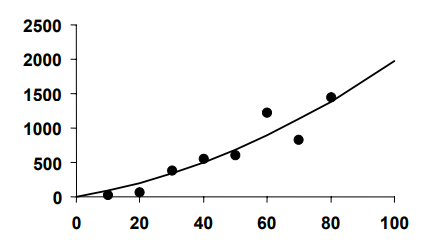
\includegraphics[width=0.5\linewidth]{fig_13_2}
		\label{fig:fig_13_2}
	\end{figure}
	\bigbreak



\section{}
The data can be tabulated and the sums computed as
	\bigbreak
	\begin{tabular}{ccccccccccc}
	\Xhline{1.5pt}i&x&y&$x^2$&$x^3$&$x^4$&$x^5$&$x^6$&xy&$x^2y$&$x^3y$\\
	\hline 1&3&1.6&9&27&81&243&729&4.8&14.4&43.2\\
		2&4&3.6&16&64&256&1024&4096&14.4&57.6&230.4\\
		3&5&4.4&25&125&625&3125&15625&22&110&550\\
		4&7&3.4&49&343&2401&16807&117649&23.8&166.6&1166.2\\
		5&8&2.2&64&512&4096&32768&262144&17.6&140.8&1126.4\\
		6&9&2.8&81&729&6561&59049&531441&25.2&226.8&2041.2\\
		7&11&3.8&121&1331&14641&161051&1771561&41.8&459.8&5057.8\\
		8&\underline{12}&\underline{4.6}&\underline{144}&\underline{1728}&\underline{20736}&\underline{248832}&\underline{2985984}&\underline{55.2}&\underline{662.4}&\underline{7948.8}\\
		$\Sigma$&59&26.4&509&4859&49397&522899&5689229&204.8&1838.4&18164\\
	\end{tabular}
	\bigbreak
Normal equations: 
	\bigbreak
	$\begin{bmatrix}
		8&59&509&4859\\
		59&509&4859&49397\\
		509&4859&49397&522899\\
		859&49397&522899&5689229\\
	\end{bmatrix}
	\begin{Bmatrix}
		a_0\\
		a_1\\
		a_2\\
		a_3\\
	\end{Bmatrix}
	=
	\begin{Bmatrix}
	26.4\\
	204.8\\
	1838.4\\
	18164\\
	\end{Bmatrix}$
	\bigbreak
which can be solved for the coefficients yielding the following best-fit polynomial
	\bigbreak
$y = -11.4887 + 7.143817x -1.04121x^2+ 0.046676x^3$
	\bigbreak
Here is the resulting fit: 
	\bigbreak
	\begin{figure}[H]
		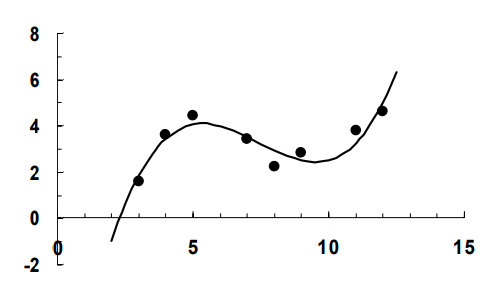
\includegraphics[width=0.5\linewidth]{fig_13_3}
		\label{fig:fig_13_3}
	\end{figure}
	\bigbreak
The predicted values can be used to determined the sum of the squares. Note that the mean
of the y values is 3.3.
	\bigbreak
	\begin{tabular}{cccccc}
	i&x&y&$y_{pred}$&$(y_i-\overline{y})^2$&$(y-\overline{y}_{pred})^2$\\
	1&3&1.6&1.83213&2.8900&0.0539\\
	2&4&3.6&3.41452&0.0900&0.0344\\
	3&5&4.4&4.03471&1.2100&0.1334\\
	4&7&3.4&3.50875&0.0100&0.0118\\
	5&8&2.2&2.92271&1.2100&0.5223\\
	6&9&2.8&2.4947&0.2500&0.0932\\
	7&11&3.8&3.23302&0.2500&0.3215\\
	8&12&4.6&4.95946&1.6900&0.1292\\
	$\Sigma$&&&&7.6000&1.2997\\
	\end{tabular}
	\bigbreak
The coefficient of determination can be computed as
	\bigbreak
$r^2=\dfrac{7.6-1.2997}{7.6}=0.829$
	\bigbreak



\section{}
\begin{lstlisting}[numbers=none]
function p = polyreg(x,y,m)
% polyreg(x,y,m):
%	 Polynomial regression.
% input:
%	 x = independent variable
%	 y = dependent variable
%	 m = order of polynomial
% output:
%	 p = vector of coefficients
n = length(x);

if length(y)~=n, error('x and y must be same length'); end
for i = 1:m+1
	for j = 1:i
		k = i+j-2;
		s = 0;
		for l = 1:n
			s = s + x(l)^k;
		end
		A(i,j) = s;
		A(j,i) = s;
	end
	s = 0;
	for l = 1:n
		s = s + y(l)*x(l)^(i-1);
	end
	b(i) = s;
end
p = A\b'; 
\end{lstlisting}
	\bigbreak
Test solving Prob. 13.3:
	\bigbreak
\begin{lstlisting}[numbers=none]
>> x = [3 4 5 7 8 9 11 12];
>> y = [1.6 3.6 4.4 3.4 2.2 2.8 3.8 4.6];
>> polyreg(x,y,3)

ans =

 -11.4887
 7.1438
 -1.0412
 0.0467 
\end{lstlisting}
	\bigbreak



\section{}
\begin{blockquote}
Because the data is curved, a linear regression will undoubtedly have too much error.
Therefore, as a first try, fit a parabola,
\end{blockquote}
	\bigbreak
\begin{lstlisting}[numbers=none]
>> format long
>> T = [0 5 10 15 20 25 30];
>> c = [14.6 12.8 11.3 10.1 9.09 8.26 7.56];
>> p = polyfit(T,c,2)

p =
 0.00439523809524	-0.36335714285714	14.55190476190477 
\end{lstlisting}
	\bigbreak
Thus, the best-fit parabola would be
	\bigbreak
$c =14.55190476 - 0.36335714T + 0.0043952381T^2$
	\bigbreak
	\begin{figure}[H]
		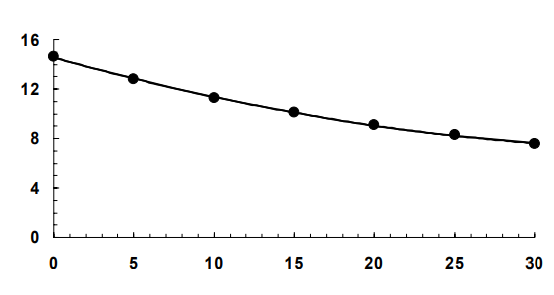
\includegraphics[width=0.5\linewidth]{fig_13_4}
		\label{fig:fig_13_4}
	\end{figure}
	\bigbreak
\begin{blockquote}
We can use this equation to generate predictions corresponding to the data. When these
values are rounded to the same number of significant digits the results are 
\end{blockquote}
	\bigbreak
	\begin{tabular}{cccc}
	\Xhline{1.5pt}T&c-data&c-pred&rounded\\
		0&14.6&14.55190&14.6\\
		5&12.8&12.84500&12.8\\
		10&11.3&11.35786&11.4\\
		15&10.1&10.09048&10.1\\
		20&9.09&9.04286&9.04\\
		25&8.26&8.21500&8.22\\
		30&7.56&7.60690&7.61\\
		\Xhline{1.5pt}
	\end{tabular}
	\bigbreak
Thus, although the plot looks good, discrepancies occur in the third significant digit.
	\bigbreak
We can, therefore, fit a third-order polynomial
	\bigbreak
\begin{lstlisting}[numbers=none]
>> p = polyfit(T,c,3)


p =
 -0.00006444444444	0.00729523809524		-0.39557936507936	14.60023809523810 
\end{lstlisting}
	\bigbreak
Thus, the best-fit cubic would be
	\bigbreak
$c =14.600238095 - 0.395579365T + 0.007295238T^2 - 0.000064444T^3$
	\bigbreak
\begin{blockquote}
We can use this equation to generate predictions corresponding to the data. When these
values are rounded to the same number of significant digits the results are 
\end{blockquote}
	\bigbreak
	\begin{tabular}{cccc}
	\Xhline{1.5pt}T&c-data&c-pred&rounded\\
		0&14.6&14.60020&14.6\\
		5&12.8&12.79663&12.8\\
		10&11.3&11.30949&11.3\\
		15&10.1&10.09044&10.1\\
		20&9.09&9.09116&9.09\\
		25&8.26&8.26331&8.26\\
		30&7.56&7.55855&7.56\\
		\Xhline{1.5pt}
	\end{tabular}
	\bigbreak
Thus, the predictions and data agree to three significant digits. 
	\bigbreak



\section{}
The multiple linear regression model to evaluate is
	\bigbreak
$o=a_{0}+a_{1} T+a_{2} c$
	\bigbreak
The [Z] and y matrices can be set up using MATLAB commands in a fashion similar to
Example 13.4,
	\bigbreak
\begin{lstlisting}[numbers=none]
>> format long
>> t = [0 5 10 15 20 25 30];
>> T = [t t t]';
>> c = [zeros(size(x)) 10*ones(size(x)) 20*ones(size(x))]';
>> Z = [ones(size(T)) T c];
>> y = [14.6 12.8 11.3 10.1 9.09 8.26 7.56 12.9 11.3 10.1 9.03 8.17
7.46 6.85 11.4 10.3 8.96 8.08 7.35 6.73 6.2]';
\end{lstlisting}
	\bigbreak
The coefficients can be evaluated as 
	\bigbreak
\begin{lstlisting}[numbers=none]
>> a = Z\y


a =
	13.52214285714286
	-0.20123809523810
	-0.10492857142857 
\end{lstlisting}
	\bigbreak
Thus, the best-fit multiple regression model is 
	\bigbreak
$o=13.52214285714286-0.20123809523810 T-0.10492857142857 c$
	\bigbreak
	We can evaluate the prediction at T = 12 and c = 15 and evaluate the percent relative error as
	\bigbreak
\begin{lstlisting}[numbers=none]
>> cp = a(1)+a(2)*12+a(3)*15


cp =
 	9.53335714285714


>> ea = abs((9.09-cp)/9.09)*100


ea =
	4.87741631305987
\end{lstlisting}
	\bigbreak
\begin{blockquote}
Thus, the error is considerable. This can be seen even better by generating predictions for
all the data and then generating a plot of the predictions versus the data. A one-to-one line
is included to show how the predictions diverge from a perfect fit. 
\end{blockquote}
	\bigbreak
	\begin{figure}[H]
		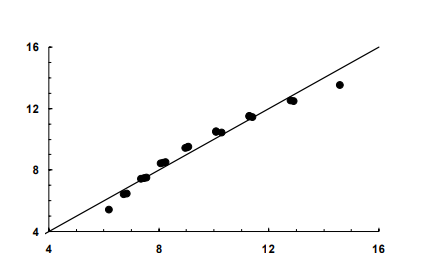
\includegraphics[width=0.5\linewidth]{fig_13_5}
		\label{fig:fig_13_5}
	\end{figure}
	\bigbreak
\begin{blockquote}
The cause for the discrepancy is because the dependence of oxygen concentration on the
unknowns is significantly nonlinear. It should be noted that this is particularly the case for
the dependency on temperature. 
\end{blockquote}
	\bigbreak



\section{}
The multiple linear regression model to evaluate is
	\bigbreak
$y=a_{0}+a_{1} T+a_{2} T^{2}+a_{3} T^{3}+a_{4} c$
	\bigbreak
The [Z] matrix can be set up as in 
	\bigbreak
\begin{lstlisting}[numbers=none]
>> T = 0:5:30;
>> T = [T T T]';
>> c = [0 0 0 0 0 0 0 10 10 10 10 10 10 10 20 20 20 20 20 20 20]';
>> o = [1 1 1 1 1 1 1 1 1 1 1 1 1 1 1 1 1 1 1 1 1]';
>> y = [14.6 12.8 11.3 10.1 9.09 8.26 7.56 12.9 11.3 10.1 9.03 8.17
7.46 6.85 11.4 10.3 8.96 8.08 7.35 6.73 6.2]';
>> Z = [o T T.^2 T.^3 c];
\end{lstlisting}
	\bigbreak
Then, the coefficients can be generated by solving Eq.(13.10) 
	\bigbreak
\begin{lstlisting}[numbers=none]
>> format long
>> a = (Z'*Z)\[Z'*y]


a =
	14.02714285714287
	-0.33642328042328
	0.00574444444444
	-0.00004370370370
	-0.10492857142857
\end{lstlisting}
	\bigbreak
Thus, the least-squares fit is 
	\bigbreak
$y=14.027143-0.336423 T+0.00574444 T^{2}-0.000043704 T^{3}-0.10492857 c$
	\bigbreak
\begin{blockquote}
The model can then be used to predict values of oxygen at the same values as the data.
These predictions can be plotted against the data to depict the goodness of fit.
\end{blockquote}
	\bigbreak
\begin{lstlisting}[numbers=none]
>> yp = Z*a
>> plot(y,yp,'o') 
\end{lstlisting}
	\bigbreak
	\begin{figure}[H]
		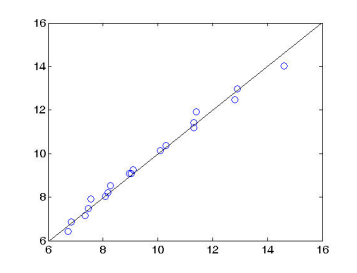
\includegraphics[width=0.5\linewidth]{fig_13_6}
		\label{fig:fig_13_6}
	\end{figure}
	\bigbreak
Finally, the prediction can be made at T = 12 and c = 15, 
	\bigbreak
\begin{lstlisting}[numbers=none]
>> a(1)+a(2)*12+a(3)*12^2+a(4)*12^3+a(5)*15
ans =
	9.16781492063485 
\end{lstlisting}
	\bigbreak
which compares favorably with the true value of 9.09 mg/L. 
	\bigbreak



\section{}
The multiple linear regression model to evaluate is 
	\bigbreak
$y=a_{0}+a_{1} x_{1}+a_{2} x_{2}$
	\bigbreak
The [Z] matrix can be set up as in 
	\bigbreak
\begin{lstlisting}[numbers=none]
>> x1 = [0 1 1 2 2 3 3 4 4]';
>> x2 = [0 1 2 1 2 1 2 1 2]';
>> y = [15.1 17.9 12.7 25.6 20.5 35.1 29.7 45.4 40.2]';
>> o = [1 1 1 1 1 1 1 1 1]';
>> Z = [o x1 x2 y];
\end{lstlisting}
	\bigbreak
Then, the coefficients can be generated by solving Eq.(13.10) 
	\bigbreak
\begin{lstlisting}[numbers=none]
>> a = (Z'*Z)\[Z'*y]


a =
	14.4609
	9.0252
	-5.7043
\end{lstlisting}
	\bigbreak
Thus, the least-squares fit is 
	\bigbreak
$y=14.4609+9.0252 x_{1}-5.7043 x_{2}$
	\bigbreak
\begin{blockquote}
The model can then be used to predict values of the unknown at the same values as the
data. These predictions can be used to determine the correlation coefficient and the standard
error of the estimate.
\end{blockquote}
	\bigbreak
\begin{lstlisting}[numbers=none]
>> yp = Z*a


>> SSR = sum((yp - y).^2)
SSR =
	4.7397


>> SST = sum((y - mean(y)).^2)
SST =
	1.0587e+003


>> r2 = (SST - SSR)/SST
r2 =
	0.9955


>> r = sqrt(r2)
r =
	0.9978


>> syx = sqrt(SSR/(length(y)-3))
syx =
	0.8888
\end{lstlisting}
	\bigbreak



\section{}
The multiple linear regression model to evaluate is
	\bigbreak
$\log Q=\log \alpha_{0}+\alpha_{1} \log (D)+\alpha_{2} \log (S)$
	\bigbreak
The [Z] matrix can be set up as is
	\bigbreak
\begin{lstlisting}[numbers=none]
>> D = [.3 .6 .9 .3 .6 .9 .3 .6 .9]';
>> S = [.001 .001 .001 .01 .01 .01 .05 .05 .05]';
>> Q = [.04 .24 .69 .13 .82 2.38 .31 1.95 5.66]';
>> o = [1 1 1 1 1 1 1 1 1]';
>> Z = [o log10(D) log10(S)] 
\end{lstlisting}
	\bigbreak
Then, the coefficients can be generated by solving Eq.(13.10)
\begin{lstlisting}[numbers=none]
>> a = (Z'*Z)\[Z'*log10(Q)]
a =
	1.5609
	2.6279
	0.5320 
\end{lstlisting}
	\bigbreak
Thus, the least-squares fit is
	\bigbreak
$\log Q=1.5609+2.6279 \log (D)+0.5320 \log (S)$
	\bigbreak
Taking the inverse logarithm gives
	\bigbreak
$Q=10^{1.5609} D^{2.6279} S^{0.5320}=36.3813 D^{2.6279} S^{0.5320}$
	\bigbreak



\section{}
The linear regression model to evaluate is
	\bigbreak
$p(t)=A e^{-1.5 t}+B e^{-0.3 t}+C e^{-0.05 t}$
	\bigbreak
The unknowns can be entered and the [Z] matrix can be set up as in
	\bigbreak
\begin{lstlisting}[numbers=none]
>> p = [7 5.2 3.8 3.2 2.5 2.1 1.8 1.5 1.2 1.1]';
>> t = [0.5 1 2 3 4 5 6 7 8 9]';
>> Z = [exp(-1.5*t) exp(-0.3*t) exp(-0.05*t)];
\end{lstlisting}
	\bigbreak
Then, the coefficients can be generated by solving Eq.(13.10)
	\bigbreak
\begin{lstlisting}[numbers=none]
>> Z = [exp(-1.5*t) exp(-0.3*t) exp(-0.05*t)];
>> a = (Z'*Z)\[Z'*p]
a =
	3.7778
	4.3872
	1.3775 
\end{lstlisting}
	\bigbreak
Thus, the least-squares fit is
	\bigbreak
$p(t)=3.7778 e^{-1.5 t}+4.3872 e^{-0.3 t}+1.3775 e^{-0.05 t}$
	\bigbreak
The fit and the data can be plotted as
\begin{lstlisting}[numbers=none]
>> pp = Z*a
>> plot(t,p,'o',t,pp)
\end{lstlisting}
	\bigbreak
	\begin{figure}[H]
		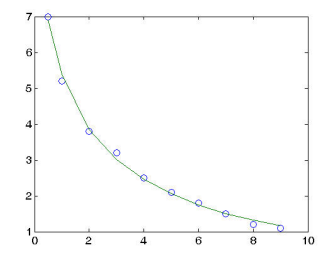
\includegraphics[width=0.5\linewidth]{fig_13_7}
		\label{fig:fig_13_7}
	\end{figure}
	\bigbreak



\section{}
First, an M-file function must be created to compute the sum of the squares,
\begin{lstlisting}[numbers=none]
function f = fSSR(a,Im,Pm)
Pp = a(1)*Im/a(2).*exp(-Im/a(2)+1);
f = sum((Pm-Pp).^2); 
\end{lstlisting}
	\bigbreak
The data can then be entered as
	\bigbreak
\begin{lstlisting}[numbers=none]
>> I = [50 80 130 200 250 350 450 550 700];
>> P = [99 177 202 248 229 219 173 142 72]; 
\end{lstlisting}
	\bigbreak
The minimization of the function is then implemented by 
	\bigbreak
\begin{lstlisting}[numbers=none]
>> a = fminsearch(@fSSR, [200, 200], [], I, P)


a =
	238.7124 221.8239
\end{lstlisting}
	\bigbreak
The best-fit model is therefore
	\bigbreak
$P=238.7124 \dfrac{I}{221.8239} e^{-\dfrac{I}{221.8239}+1}$
	\bigbreak
The fit along with the data can be displayed graphically.
	\bigbreak
\begin{lstlisting}[numbers=none]
>> Pp = a(1)*I/a(2).*exp(-I/a(2)+1);
>> plot(I,P,'o',I,Pp) 
\end{lstlisting}
	\bigbreak
	\begin{figure}[H]
		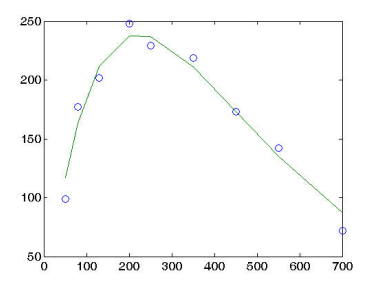
\includegraphics[width=0.5\linewidth]{fig_13_8}
		\label{fig:fig_13_8}
	\end{figure}
	\bigbreak



\section{}
First, an M-file function must be created to compute the sum of the squares,
	\bigbreak
\begin{lstlisting}[numbers=none]
function f = fSSR(a,xm,ym)
yp = a(1)*xm.*exp(a(2)*xm);
f = sum((ym-yp).^2); 
\end{lstlisting}
	\bigbreak
The data can then be entered as
\begin{lstlisting}[numbers=none]
>> x = [.1 .2 .4 .6 .9 1.3 1.5 1.7 1.9];
>> y = [0.75 1.25 1.45 1.25 0.85 0.55 0.35 0.28 0.18]; 
\end{lstlisting}
	\bigbreak
The minimization of the function is then implemented by
	\bigbreak
\begin{lstlisting}[numbers=none]
>> a = fminsearch(@fSSR, [1, 1], [], x, y)


a =
	9.8545 -2.5217 
\end{lstlisting}
	\bigbreak
The best-fit model is therefore
	\bigbreak
$y=9.8545 x e^{-2.5217 x}$
	\bigbreak
The fit along with the data can be displayed graphically.
	\bigbreak
\begin{lstlisting}[numbers=none]
>> yp = a(1)*x.*exp(a(2)*x);
>> plot(x,y,'o',x,yp) 
\end{lstlisting}
	\bigbreak
	\begin{figure}[H]
		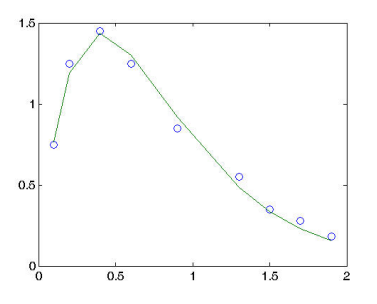
\includegraphics[width=0.5\linewidth]{fig_13_9}
		\label{fig:fig_13_9}
	\end{figure}
	\bigbreak



\section{}
\begin{enumerate}[label=\bfseries(\alph*)]
\item The model can be linearized by inverting it,
	\bigbreak
$\dfrac{1}{v_{0}}=\dfrac{K}{k_{m}} \dfrac{1}{[S]^{3}}+\dfrac{1}{k_{m}}$
	\bigbreak
If this model is valid, a plot of $1 / v_{0}$ versus $1 /[S]^{3}$ should yield a straight line with a slope of $K / k_{m}$ and an intercept of $1 / k_{m}$. The slope and intercept can be implemented in MATLAB using the M-file function linregr (Fig. 12.12),
	\bigbreak
\begin{lstlisting}[numbers=none]
>> S = [.01 .05 .1 .5 1 5 10 50 100];
>> v0 = [6.078e-11 7.595e-9 6.063e-8 5.788e-6 1.737e-5 2.423e-5
2.43e-5 2.431e-5 2.431e-5];
>> a = linregr(1./S.^3,1./v0)


a =
	1.0e+004 *
	1.64527391375701 4.13997346408367 
\end{lstlisting}
	\bigbreak
These results can then be used to compute $k_{m}$ and $K$,
	\bigbreak
\begin{lstlisting}[numbers=none]
>> km=1/a(2)
km =
	2.415474419523452e-005


>> K=km*a(1)
K =
	0.39741170517893
\end{lstlisting}
	\bigbreak
Thus, the best-fit model is 
	\bigbreak
$v_{0}=\dfrac{2.415474 \times 10^{-5}[S]^{3}}{0.39741+[S]^{3}}$
	\bigbreak
The fit along with the data can be displayed graphically. We will use a log-log plot because
of the wide variation of the magnitudes of the values being displayed, 
	\bigbreak
\begin{lstlisting}[numbers=none]
>> v0p = km*S.^3./(K+S.^3);
>> loglog(S,v0,'o',S,v0p) 
\end{lstlisting}
	\bigbreak
	\begin{figure}[H]
		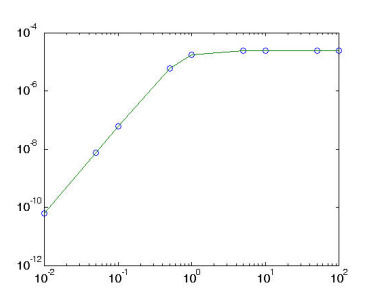
\includegraphics[width=0.5\linewidth]{fig_13_10}
		\label{fig:fig_13_10}
	\end{figure}
	\bigbreak
\item An M-file function must be created to compute the sum of the squares, 
\end{enumerate}
\begin{lstlisting}[numbers=none]
function f = fSSR(a,Sm,v0m)
v0p = a(1)*Sm.^3./(a(2)+Sm.^3);
f = sum((v0m-v0p).^2); 
\end{lstlisting}
	\bigbreak
The data can then be entered as
	\bigbreak
\begin{lstlisting}[numbers=none]
>> S = [.01 .05 .1 .5 1 5 10 50 100];
>> v0 = [6.078e-11 7.595e-9 6.063e-8 5.788e-6 1.737e-5 2.423e-5
2.43e-5 2.431e-5 2.431e-5]; 
\end{lstlisting}
	\bigbreak
The minimization of the function is then implemented by 
\begin{lstlisting}[numbers=none]
>> format long
>> a = fminsearch(@fSSR, [2e-5, 1], [], S, v0)


a =
	0.00002430998303 0.39976314533880 
\end{lstlisting}
	\bigbreak
The best-fit model is therefore
	\bigbreak
$v_{0}=\dfrac{2.431 \times 10^{-5}[S]^{3}}{0.399763+[S]^{3}}$
	\bigbreak
\begin{blockquote}
The fit along with the data can be displayed graphically. We will use a log-log plot because
of the wide variation of the magnitudes of the values being displayed,
\end{blockquote}
	\bigbreak
\begin{lstlisting}[numbers=none]
>> v0p = a(1)*S.^3./(a(2)+S.^3);
>> loglog(S,v0,'o',S,v0p) 
\end{lstlisting}
	\begin{figure}[H]
		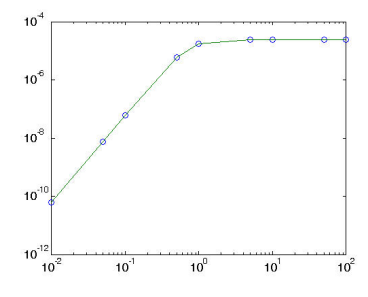
\includegraphics[width=0.5\linewidth]{fig_13_11}
		\label{fig:fig_13_11}
	\end{figure}
	\bigbreak
\end{document}